\chapter{Background}
This chapter reviews the theories necessary for the main part of the thesis. As we are creating topic models of pretrained language models, we need to know what those are and how they work. In the following sections, we explore their relevant origin  on top of providing an overview on current evaluation and comparison techniques.

% =============================
\section{Language Modeling}
% =============================
\subsection{Definition and Application}
Language models are created to distill valuable insights from raw text without the help of a human. To name a few tasks of language models:
\begin{itemize}
    \item \textbf{Natural-language generation (NLG)} extracts and transforms information in the form of raw data or text into readable and human understandable text. 
    \item \textbf{Natural-language understanding (NLU)} takes text as input and translates it into a more formal representation, so that computer applications can understand it. For example simple commands given to robots or more complex ones, like comprehension of newspaper articles.
    \item \textbf{Automatic summarization of texts} produces a readable summary of a fragment of text and can be extractive or abstractive. Extractive summarization concatenates strings with different length without knowing what they actually mean. On the other hand, abstractive summarization creates a context sensitive summary by using a combination of statistical and linguistic properties of the analyzed text. \cite{gupta2010survey}
    \item \textbf{Machine translation} translates text or speech from one language to another.
    \item \textbf{Question answering}, with or without context, answers text questions from humans. Answers are created with knowledge from large databases. This is usually a knowledge database or an unstructured collection of natural language documents. The questions themselves can be closed or open-ended.
    \item \textbf{Speech recognition} creates text equivalent to any input in the form of audio speech. 
    \item \textbf{Optical character recognition (OCR)} scans visual input and transforms it into machine-encoded text. Such input can be to images of typed, handwritten or printed text in the from a scanned document, a photo of a document or a scene-photo.
    \item \textbf{Paraphrasing} is a subcategory of text-to-text generation and is the art of paraphrasing words, sentences and full texts.
\end{itemize}

The standard definition of a language model is a model of the probability distribution over strings $p(\mathbf{y})$ in a natural language. This model should provide an estimate of the (unconditional) probability of observing some string $\mathbf{y} \in\mathcal{Y}$, where $\mathcal{Y}$ is the set of all valid strings in a language. Different attempts over time resulted in different model architectures, e.g. the n-gram (unigram, bigram, trigram, etc.) model, the log-linear model and the neural model. For large pretrained language models, neural language models deliver state of the art results on various NLP tasks. Compared to traditional language models, neural models allow conditioning on increasingly larger contexts with only linear increases in the number of parameters. They parameterize words as vectors (word embeddings) and use these vectors as inputs. These parameters are learned as part of the training process of neural models. Each neural model has a specifically designed architecture for the data it was designed to learn, which puts restrictions on the learning algorithm. Furthermore, the ability to generalize to unseen data introduces an inductive bias to our model, which in itself is not a bad thing. In fact, we need our model to generalize to unseen data. This way, the model will be able to apply the learned knowledge to different subtasks it was not trained for, e.g. prediction of news articles or movie reviews.

A first attempt to neural language modeling by Bengio et al., 2003 \cite{bengio2003neural} uses feed-forward neural network models. However, with increasing lexicon size, the computations regarding the output layer become computationally intractable. The reason being that the predicted output on a particular input needs to be a probability distribution over the entire lexicon (softmax over the vocabulary). With recurrent neural networks (RNN), this limitation is avoided as they can learn arbitrary long influences without being dependant on the size of the lexicon (infinite context). In an RNN, each node is aware of its direct predecessor and the information from earlier nodes is only indirectly available through the encoding of the encodings. This leads to a loss of information as the lexicon gets bigger.

% =======================================
\subsection{Attention Mechanism}
The attention mechanism poses a solution to the loss of information in large RNN networks. It overcomes the limitation of the fixed-size vector representation of the input sequence. Attention comes in the form of a hidden layer and computes a categorical distribution (or hierarchy of categorical distributions) over the input. The input can be the direct words or intermediate input from other layers. \cite{kim2017structured}

The concept of the attention mechanism was introduced by Bahadanau et al., 2014 \cite{bahdanau2014neural} for machine translation (see fig. \ref{fig:attentionMT}) and has demonstrated success on various NLP tasks. 
\begin{figure}[H]
    \centering
    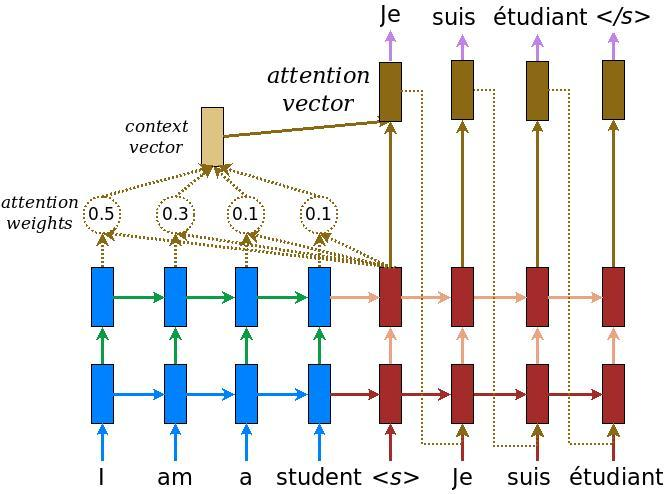
\includegraphics[width=0.7\textwidth]{figures/attention}
    \caption{Attention Mechanism for machine translation with encoder (blue) and decoder (red). \cite{attentionmechanism}}
    \label{fig:attentionMT}
\end{figure}
Later, Yang et al., 2016 \cite{yang2016hierarchical} introduced the intra or self-attention mechanism for document classification. Because not all words contribute equally to the representation of the meaning of a sentence, the attention mechanism was adapted to a word level, such that it relates different positions of a single sequence to compute a representation of the sequence. 

Vaswani et al., 2017 \cite{vaswani2017attention} exploited this technique in their proposed architecture, the Transformer, and introduced an adaptation of self-attention and the new multi-head attention. 

% =======================================
\subsubsection{Self-Attention}
The self-attention mechanism \cite{vaswani2017attention} makes inputs aware of each other and tells them which are the more important ones. The outputs of this mechanism are aggregates of these interactions and the attention scores. Every input is represented by three vectors, i.e. a key $k$, a query $q$ and a value $v$. They are a product of the input vector and three global weight matrices, i.e. $W^Q,\;W^K,\;W^V$ (see fig. \ref{fig:selfattention}), which are learned during the training process. Every input uses those matrices to calculate their three representations.
\begin{figure}[H]
    \centering
    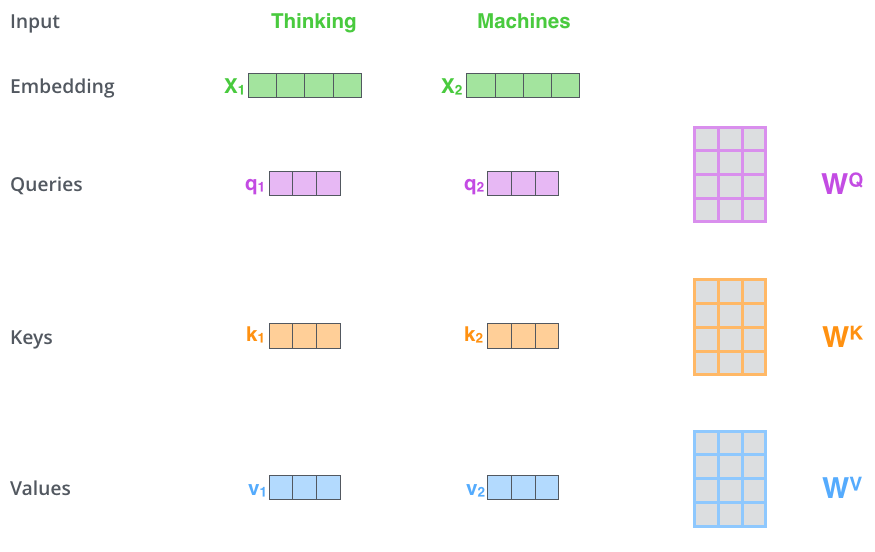
\includegraphics[width=0.7\textwidth]{figures/selfattention}
    \caption{Self-Attention Mechanism: Illustrating input/embeddings (green), query (pink), keys (orange) and values (blue). \cite{illustratedtransformer}}
    \label{fig:selfattention}
\end{figure}
Depending on where to put attention, different scoring functions are used. In the Transformer architecture, the scaled-dot-product (see fig. \ref{fig:scaled-dot-product-attention}) is used.
\begin{figure}[H]
    \centering
    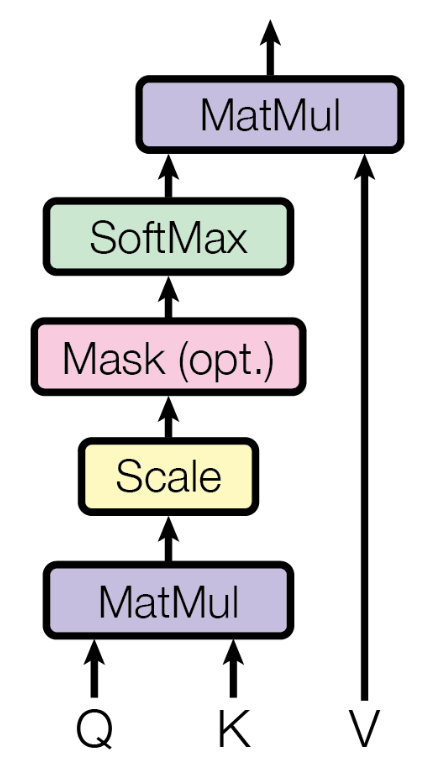
\includegraphics[width=0.2\textwidth]{figures/scaled-dot-product-attention}
    \caption{Scaled Dot-Product. \cite{vaswani2017attention}}
    \label{fig:scaled-dot-product-attention}
\end{figure}
The output of the scaled-dot-product attention are the weighted values $V$ according to eq. \ref{eq:sdp}. 
\begin{equation}\label{eq:sdp}
    \text{Attention}(\mathbf{Q},\mathbf{K},\mathbf{V})=\text{softmax}\left(\frac{\mathbf{Q}\mathbf{K}^T}{\sqrt{d_k}}\right)\mathbf{V}
\end{equation}

% =======================================
\subsubsection{(Masked) Multi-Head Attention}\label{sec:multheadat}
the goal is to make the different inputs aware of each other at different positions. Apart from the collectively learned weight matrices ($W^Q,\;W^K,\;W^V$), we calculate the output for input $x_1$ by using the query vector $q_1$ in all self-attentions instead of using each their own query vector ($q_2, q_3, ...)$. The resulting self-attention vectors are then summed up giving us the multi-head attention vector for input $x_1$. This process is repeated for every input, but in practice, this is done very efficiently with matrix multiplications (see fig. \ref{fig:multi-head-attention}).
\begin{figure}[H]
    \centering
    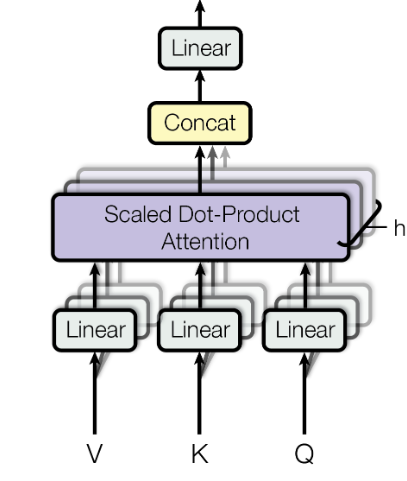
\includegraphics[width=0.3\textwidth]{figures/multi-head-attention}
    \caption{Multi-Head Attention. \cite{vaswani2017attention}}
    \label{fig:multi-head-attention}
\end{figure}

The masked multi-head attention is a slight variation of the normal multi-head attention. Before the softmax step (see fig. \ref{fig:scaled-dot-product-attention}), the multi-head-attention layer uses only earlier positions in the output sequence. This is done by setting all future positions to minus infinity. 

% =======================================
\subsection{The Transformer}
Vaswani et al., 2017 \cite{vaswani2017attention} posed a solution, to the limitations of the RNN architectures by combining original attempts to neural language modeling, which were based on feed-forward networks, with the attention mechanism. The so called Transformer architecture relies entirely on the attention mechanism to draw out the global dependencies between the input and output \cite{illuaatte}. It predicts $y_t$ by only using the $k$ most recent inputs, $x_{t-k+1},...,x_t$ (fig. \ref{fig:feedforward0}). To be able to depend on the most $k$ recent inputs, the model must assume a strong conditional independance.
\begin{figure}[H]
    \centering
    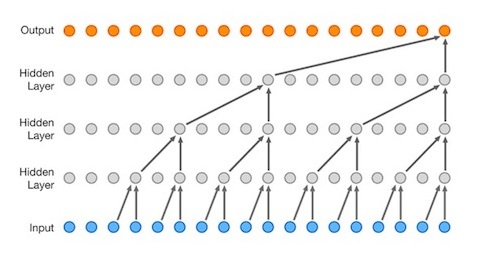
\includegraphics[width=0.9\textwidth]{figures/feedforward0}
    \caption{Illustration of an autoregressive feed-forward language model. \cite{feedforward}}
    \label{fig:feedforward0}
\end{figure}
Please note that in the next step the output is generated conditioned on the $k$ most recent inputs and becomes part of the input. The window of $k$ inputs then shifts one step to the right (fig. \ref{fig:feedforward1}).
\begin{figure}[H]
    \centering
    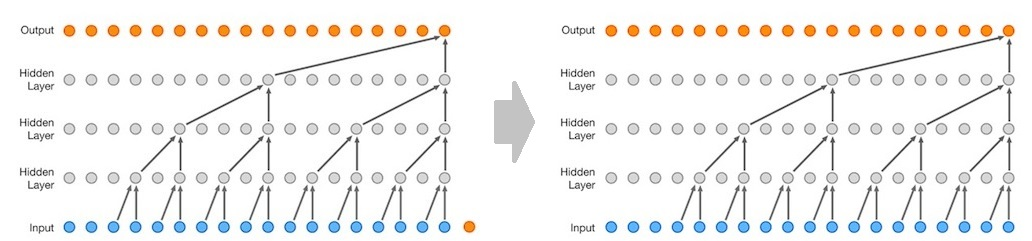
\includegraphics[width=1.0\textwidth]{figures/feedforward1}
    \caption{Illustration of the next step of an autoregressive feed-forward language model. \cite{feedforward}}
    \label{fig:feedforward1}
\end{figure}
The originally proposed Transformer architecture (see fig. \ref{fig:transformer-vis}) is an alteration of the sequence-to-sequence or encoder-decoder model \cite{attentionmechanism}. 
\begin{figure}[H]
    \centering
    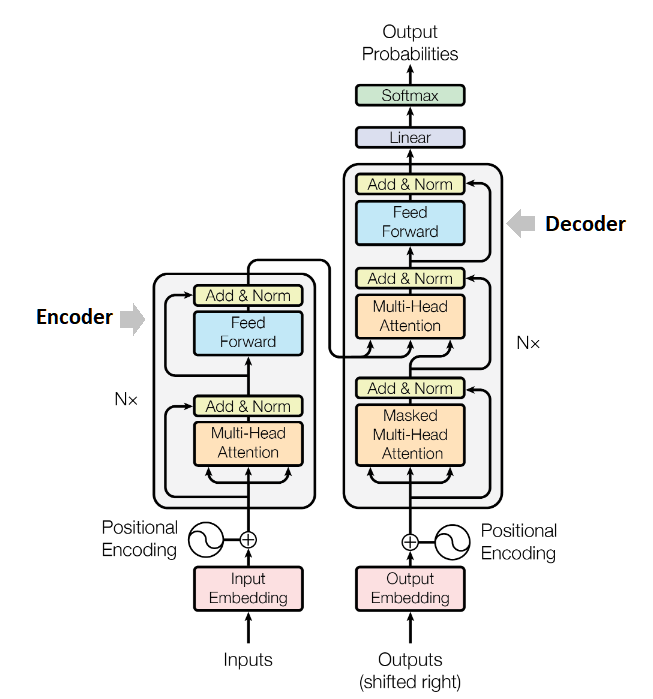
\includegraphics[width=0.7\textwidth]{figures/transformer}
    \caption{Illustration of the original Transformer Architecture. \cite{vaswani2017attention}}
    \label{fig:transformer-vis}
\end{figure}
Fig. \ref{fig:transformer-vis} just visualizes the incorporation of one encoder and one decoder. In practice, multiple encoders and decoders are put in series (see fig. \ref{fig:transformer-mult}).
\begin{figure}[H]
    \centering
    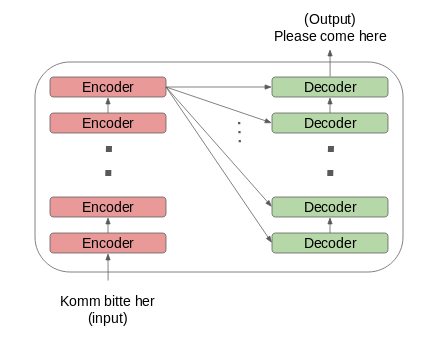
\includegraphics[width=0.6\textwidth]{figures/mult_trafo}
    \caption{Illustration of the encoder-decoder stack. \cite{howdotrafo}}
    \label{fig:transformer-mult}
\end{figure}
We can see that first the learned embeddings get encoded with a positional encoding. This is done by adding a one-hot vector to the embedding, which indicates the position of each word. 

The encoder encodes the full sequence into a context vector with fixed length. It is doing that by stepping through the input time steps. In the Transformer architecture this context vector comes in the form of a set of attention vectors $K$ and $V$. 

The decoder steps through the output time steps. While doing that, it reads from the two attention vectors, $K$ and $V$, mentioned before. These are used by each decoder in its \textit{Multi-Head Attention} (see sec. \ref{sec:multheadat}) block and help the decoder focus on appropriate places in the input sequence. After multiple decoding steps, the output after a linear and softmax block is a probability distribution where a word is sampled from (see sec. \ref{sec:gentext}). The sampled word of each iteration is then appended to the original input and again fed into the decoder to calculate the next output, and so on. Just like with the encoder inputs, the positional encodings are added to the word embeddings at every iteration. 

After basic training or pretraining, the language model is usually fine-tuned for specific NLP tasks. Fine-tuning means training on a task-specific dataset. Depending on performance and task, additional linear layers are added at the end of the language model and some parameters of the model are frozen, i.e. they do not change while fine-tuning. \cite{trafoarch}

% =======================================
\subsection{Transformer Based Architectures}
The realization that the encoder and decoder part can be used separately for different NLP tasks led to different language models based on the Transformer architecture. 

% =======================================
\subsubsection{GPT-1}
Focusing research on the decoder part (see fig. \ref{fig:gpt}) resulted in the well-known GPT-1 model \cite{radford2018improving}. GPT-1 computes the probability $p(\mathbf{y})$ of a complete sentence given nothing or a beginning of a sentence, where $\mathbf{y}\in\mathcal{Y}$ and $\mathcal{Y} = \{\textsc{bos}+\mathbf{v}+\textsc{eos}\mid \mathbf{v} \in \mathcal{V}^* \}$. $\mathbf{y}= \langle y_1, y_2, \dots\rangle$ is a sequence consisting of natural language tokens  $y\in\mathcal{V}$ from a set vocabulary $\mathcal{V}$, padded with special \textsc{bos} and \textsc{eos} tokens to demarcate the beginning and end of a string, respectively. 
\begin{figure}[H]
    \centering
    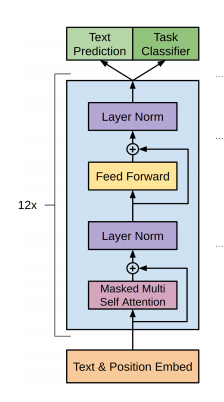
\includegraphics[width=0.3\textwidth]{figures/gptarch}
    \caption{The GPT-1 Architecture. \cite{radford2018improving}}
    \label{fig:gpt}
\end{figure}
GPT-1 is a unidirectional model, meaning it is only aware of what came before. It learns using unlabeled data and is fine-tuned by providing examples of specific downstream tasks like classification, sentiment analysis, textual entailment, etc. Its major advantage is the massive volume of data it was pretrained on. This makes adapting the \textit{raw}-trained model possible for different NLP tasks with very little data. 

% =======================================
\subsubsection{GPT-2}
The GPT-2 \cite{gpt-2} model pretty much follows the architecture of the original GPT-1 model (see fig. \ref{fig:gpt2}). New additions are that each sub-block now has the layer normalization from the end in the beginning and to the layer normalization block in the middle an additional layer is added (see fig. \ref{fig:gpt2}). The weights of the residual layers (used at initialization) are newly scaled by a factor of $1/\sqrt{N}$ where $N$ is the number of residual layers. This accounts for the accumulation on the residual path with model depth. The vocabulary is expanded to 50,257 tokens, the context size to 1024 tokens and the batchsize to 512 documents \cite{gpt-2}. This resulted in 1.5B parameters for the largest model in contrast to the 117M parameters for GPT-1. 
\begin{figure}[H]
    \centering
    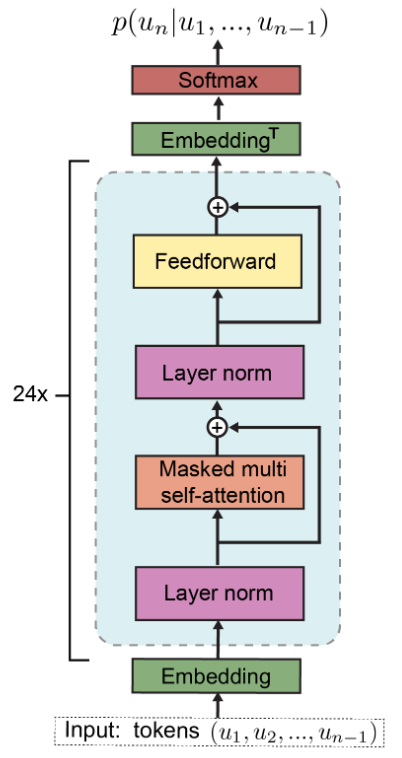
\includegraphics[width=0.4\textwidth]{figures/gpt2}
    \caption{The GPT-2 Architecture. \cite{heilbron2019tracking}}
    \label{fig:gpt2}
\end{figure}
The model was trained on the WebText dataset \cite{radford2019language}. This dataset was created by scraping web pages which have been curated, respectively filtered, by humans and then filtered with a combination of content extractors. Important to note is that Wikipedia was not included as it is a common data source for other datasets and could complicate analysis due to overlapping training data with test evaluation tasks. \cite{gpt-2}

% =======================================
\subsubsection{Transformer-XL}
Transformer-XL \cite{transformer-xl} builds upon the decoder part of the Transformer architecture. It extends the memory of the fixed-length context by conditioning on the sequences that came before. Without disrupting temporal coherence, Transformer-XL additionally solves the issue of context fragmentation. Context fragmentation is one of the main limitations of the original Transformer model and happens when a model tries to fit a document, the document gets segmented because it is too big, and long-term dependencies are then lost. 

The decoder from the original Transformer architecture is modified as such, that it functions like a cell from the RNN architecture where the memory transfer happens in the attention mechanism (see fig. \ref{fig:transformer-xl-arch}).
\begin{figure}[H]
    \centering
    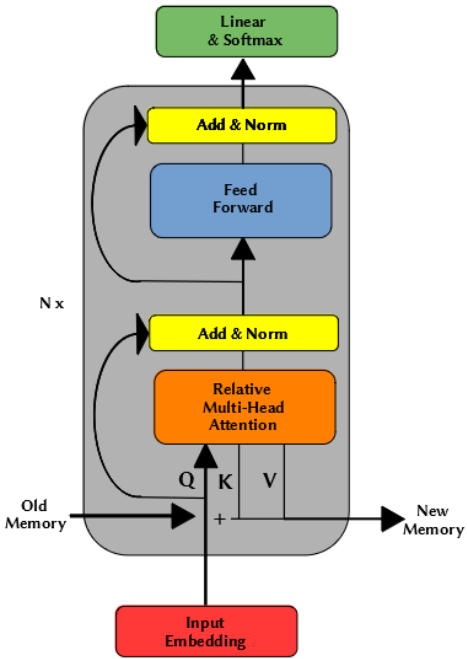
\includegraphics[width=0.5\textwidth]{figures/transformer-xl-arch}
    \caption{The Transformer-XL model. \cite{dowdell2020language}}
    \label{fig:transformer-xl-arch}
\end{figure}
Transformer-XL was trained separately on multiple datasets including Wikitext-103 and experiments have shown that it learns much longer dependencies.

% =======================================
\subsubsection{Probing Language Models}
A language model tries to learn the hidden structures and connections between sentences and words in the training corpus. To shed light on these hidden properties, researchers try to isolate linguistic phenomena through specifically designed multi-class classification problems, so called probing tasks. We assume that if a system has a good performance on a probing task, it has encoded the phenomena we were probing for. Those probes can have a low computational cost but there is a hidden complexity, i.e. we do not know the ideal setup. This means, we do not know how complex our probe has to be to find a property, e.g. whether a linear model suffices or deep learning is required. Thus, what part of the training data we use for training the probe, is rather unclear. We know in fact that with enough training data, a complex enough model is able to learn any linguistic phenomena we want it to find, and we therefore have to be aware of false positives. Recent studies have shown that it is definitely possible to memorize a good amount of specific labeling decisions without being dependant on the representation's linguistic properties. \cite{desintpro, gul2019linspector, hewitt2019structural, white2021non, lingwis}

% =======================================
\section{Generating Text From Pretrained Models}\label{sec:gentext}
% =======================================
\subsection{Ancestral Sampling}\label{sec:sampling}
Based on the standard definition of a language model and therefore on an autoregressive language model $p_\theta$, a string $\mathbf{y}\sim p_\theta$ can be generated from the conditional probability distributions. Given the relationship in eq. \ref{eq:joint}, we can set $y_1 = \textsc{bos}$ or the empty string, and sample $y_t\sim p(\cdot\mid\mathbf{y}_{<t})$ until we sample the \textsc{eos} token. 
\begin{equation}\label{eq:joint}
    p(\mathbf{y})=p(y_1,...,y_t)=p(y_1)\cdot p(y_2\mid y_1)\cdot...\cdot p(y_t\mid y_{t-1})=\prod_{t=1}^{|\mathbf{y}|} p(y_t\mid\mathbf{y}_{<t})
\end{equation}
This means, using the chain rule of probability, we can model the probability of an entire string as the product of the conditional probability of each word given its prior context. Here we define $\mathbf{y}_{<t} = \langle y_1, \dots, y_{t-1}\rangle$. We call this ancestral sampling, as we start by sampling the ancestor $p(y_1)$, then $p(y_2\mid y_1)$ and so on.

% =======================================
\subsection{Top-P Sampling}
In Top-P or \textit{nucleus} sampling \cite{holtzman2019curious} we choose from the smallest possible set of words whose cumulative probability exceeds the probability $p$. Among this set of words, the probability mass is redistributed. Thus, the number of words in the set can dynamically increase and decrease according to the probability distribution of the next word.

Formally, Top-P sampling reduces the set of words $\mathcal{V}$ from the distribution $p(y\mid y_{1:i-1})$ to the smallest subset $\mathcal{V}^{(p)}\subset \mathcal{V}$, s.t.
\begin{equation}
    \sum_{y\in \mathcal{V}^{(p)}}{p(y\mid y_{1:i-2})}\geq p.
\end{equation}
Illustrated by an example in fig. \ref{fig:topp}, we set $p=0.93$. Top-P sampling chooses the minimum number of words, such that their summed up probability mass exceeds $p=93\%$. Here, this set is defined as $\mathcal{V}_{top-p}$ (per definition, equal to $\mathcal{V}^{(0.93)}$). On the left side the 9 most likely words have to be included, where on the right side only the top 3 words are needed to exceed $93\%$. \cite{trafogen}
\begin{figure}[H]
    \centering
    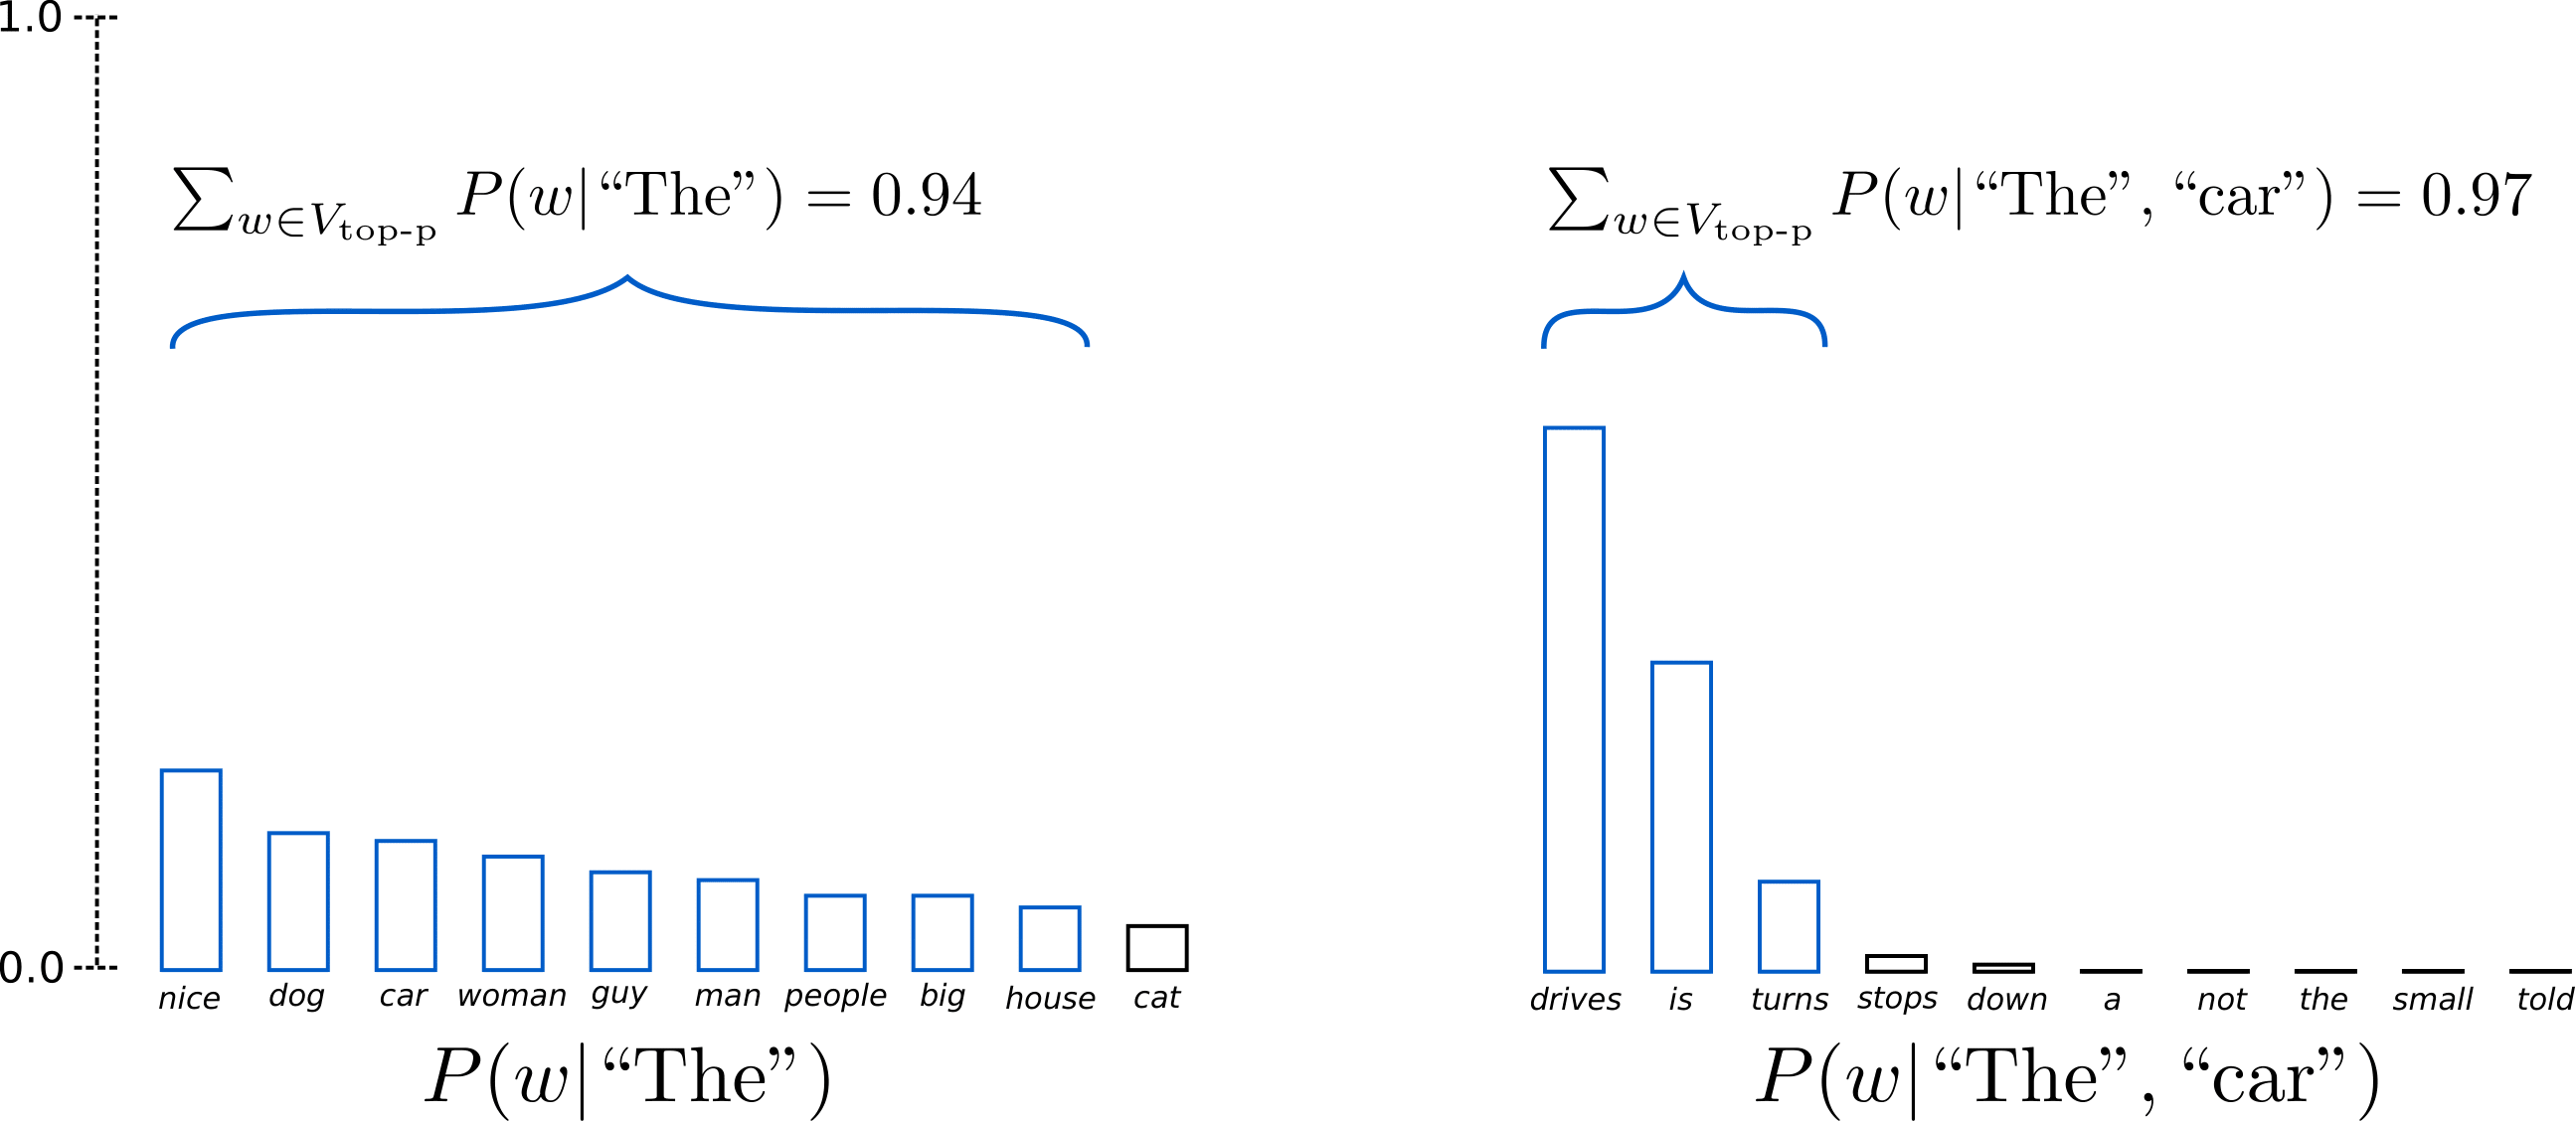
\includegraphics[width=1.0\textwidth]{figures/topp}
    \caption{Top-P sampling example. \cite{trafogen}}
    \label{fig:topp}
\end{figure}

% =======================================
\subsection{Typical Sampling}
Typical sampling \cite{meister2022typical} tries to imitate human communication. Instead of choosing words that have a certain probability mass, like Top-P sampling, it samples according to the information content of the words. The information content of the set of words is expected to be close to the information content of the model. Which is equal to its conditional entropy, i.e. we assume that for human-like text eq. \ref{eq:toppdiff} is very small.
\begin{equation}
    \varepsilon=\left|H(p(\cdot\mid \mathbf{y}_{<t}))+log\, p(y_t\mid \mathbf{y}_{<t})\right|
\label{eq:toppdiff}
\end{equation}
The sampled distribution is then limited to the word subset as $\mathcal{V}^{(\tau)}\subseteq\mathcal{V}$. This subset has to minimize eq. \ref{eq:toppdiff2} at each time step. Therefore, the subset changes constantly. 
\begin{equation}
    \sum_{y\in\mathcal{V}^{(\tau)}}{\varepsilon},\text{ s.t. }\sum_{y\in\mathcal{V}^{(\tau)}}{p(y\mid \mathbf{y}_{<t})}\geq\tau.
\label{eq:toppdiff2}
\end{equation}
After reducing the word count in the subset, it has to be renormalized according to eq. \ref{eq:norm}.
\begin{equation}
    \begin{aligned}
        \pi(y\mid\mathbf{y}_{<t})=\left\{
        \begin{matrix*}[l]
            p(y\mid\mathbf{y}_{<t})/\sum_{y\in\mathcal{V}^{(\tau)}}{p(y\mid\mathbf{y}_{<t})}, & \text{if }y\in \mathcal{V}^{(k)} \\ 
            0, & \text{else}
        \end{matrix*}\right.
    \end{aligned}
\label{eq:norm}
\end{equation}

% =======================================
\subsection{Evaluation and Metrics}
In general, it is a good idea not only to evaluate our trained model by the loss or the accuracy, but also by testing them on an actual task. We call that extrinsic evaluation. By embedding our trained model directly in an application and measuring how much the application improves, we can immediately see how different models perform and behave. For example, if we want to measure the difference in performance of two models trained for speech recognition. To achieve that, we run the speech recognizer two times and can then directly see which one of the results is a more accurate transcription. This process requires us to train a full system, which makes it computationally expensive and, depending on your model and processing power, very slow. Therefore, it is sometimes more practical to have a metric (better than accuracy or loss) that can cost-efficiently evaluate potential improvements in a language model and its quality, independent of any application. We call this intrinsic evaluation. This evaluation needs, apart from the model, a test set. The models we want to compare are then fitted onto this test set and whichever model assigns a higher probability, or rather more accurately predicts the test set, is a better model. The metric itself is based on the probability of the test set. Important is that any part of the test set should not be used for training. Otherwise, it would introduce a bias to the model which makes the probabilities for the test set higher than they actually are. An example for a widely used probability-based metric is Perplexity, or short PP. \cite{slp3}

% =======================================
\subsubsection{Perplexity}\label{sec:perplexity}
Perplexity \cite{perplexity} is an intrinsic evaluation method and is the inverse probability of the test set, normalized by the number of words. For a test set$_w=w_1,w_2,...,w_N$ the Perplexity is:
\begin{equation}
    PP(W)=\sqrt[n]{\frac{1}{P(w_1,...,w_N)}}.
    \label{eq:perplexity}
\end{equation}
To a human-like and syntactically correct text, a model assigns a high probability. Low probabilities should be the result of fake, incorrect, or highly infrequent sentences. Therefore, the best model is going to be the one that assigns the highest probability to a real and correct test set. By assigning a high probability, the model is not perplexed (surprised) by it (see fig. \ref{fig:perplexity}). This implicates that a language model with low perplexity has a good understanding of how the language works. A simpler interpretation of the perplexity score is interpreting it as the weighted branching factor. This means, if we have a perplexity of 42, the model is confused because it has to pick from 42 words when trying to guess the next word. \cite{perplexity}
\begin{figure}[H]
    \centering
    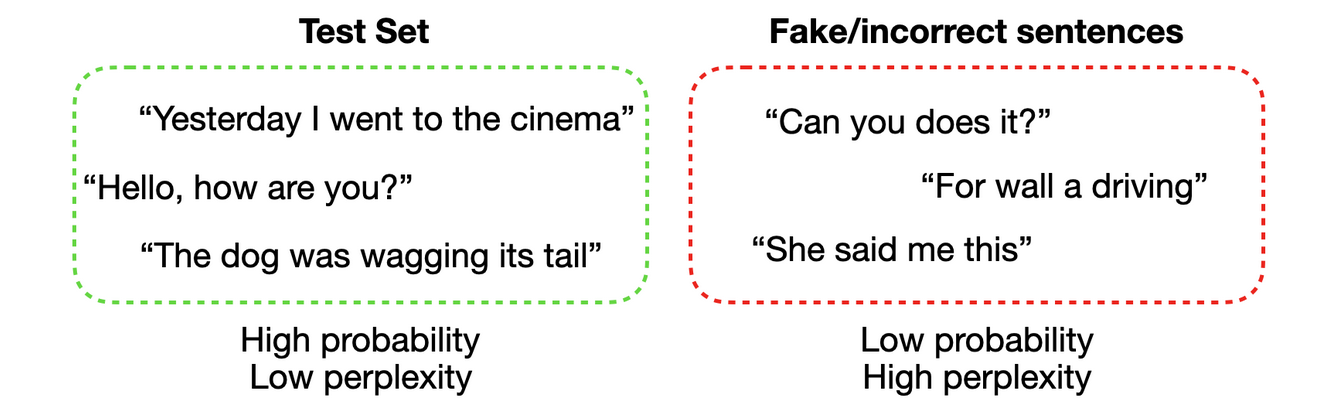
\includegraphics[width=1.0\textwidth]{figures/perplexity_example}
    \caption{Example of the Perplexity score. \cite{perplexity}}
    \label{fig:perplexity}
\end{figure}
Perplexity can also be defined as the exponential of the cross-entropy (see eq. \ref{eq:crosspp}), which is equivalent to the previous definition (eq. \ref{eq:perplexity}).
\begin{equation}
    PP(W)=2^{H(W)}=2^{-\frac{1}{N}log_2 P(w_1,...,w_N)}
\label{eq:crosspp}
\end{equation}

% =======================================
\section{Topic Modeling}
% =======================================
\subsection{Definition and Application}
A \textit{topic} is normally a phrase or a set of words that describes the content of a text. Topic modeling tries to find such topics. It is an unsupervised machine learning technique which has the ability to analyze a set of documents. Within those documents it detects patterns in multiple sentences down to the word level. It then clusters groups of words and similar expressions to best characterize this set of documents. This technique is useful for a wide range of data analysis from social media posts, emails, chats, customer support conversations, up to cancers' genomic samples. The process of dividing a corpus can in general be divided into two parts:
\begin{enumerate}
    \item A set of topics, where the topic is described in some specific way
    \item Multiple sets of grouped documents according to the topics they cover
\end{enumerate}
We assume that every document is represented by a distribution over topics. This distribution is the result of the probability mass for every topic covering this document. Those topics are defined and learned in the process, like latent variables. It is an unsupervised technique and does not require a training dataset. Hidden patterns and insights are found in the process. This does not guarantee accurate results. \cite{tmint} 

An well-known topic modeling technique is called latent Dirichlet allocation (LDA) \cite{blei2003latent}. 

% =======================================
\subsection{Latent Dirichlet Allocation (LDA)}
LDA \cite{blei2003latent} is a statistical model of a collection of documents. The model assumes that a document consists of multiple topics and a topic of multiple words. This variability of random multinomial distributions is modeled with the help of the Dirichlet distribution. The Dirichlet distribution basically models a probability distribution of probability distributions. The figure below illustrates the intuition:
\begin{figure}[H]
    \centering
    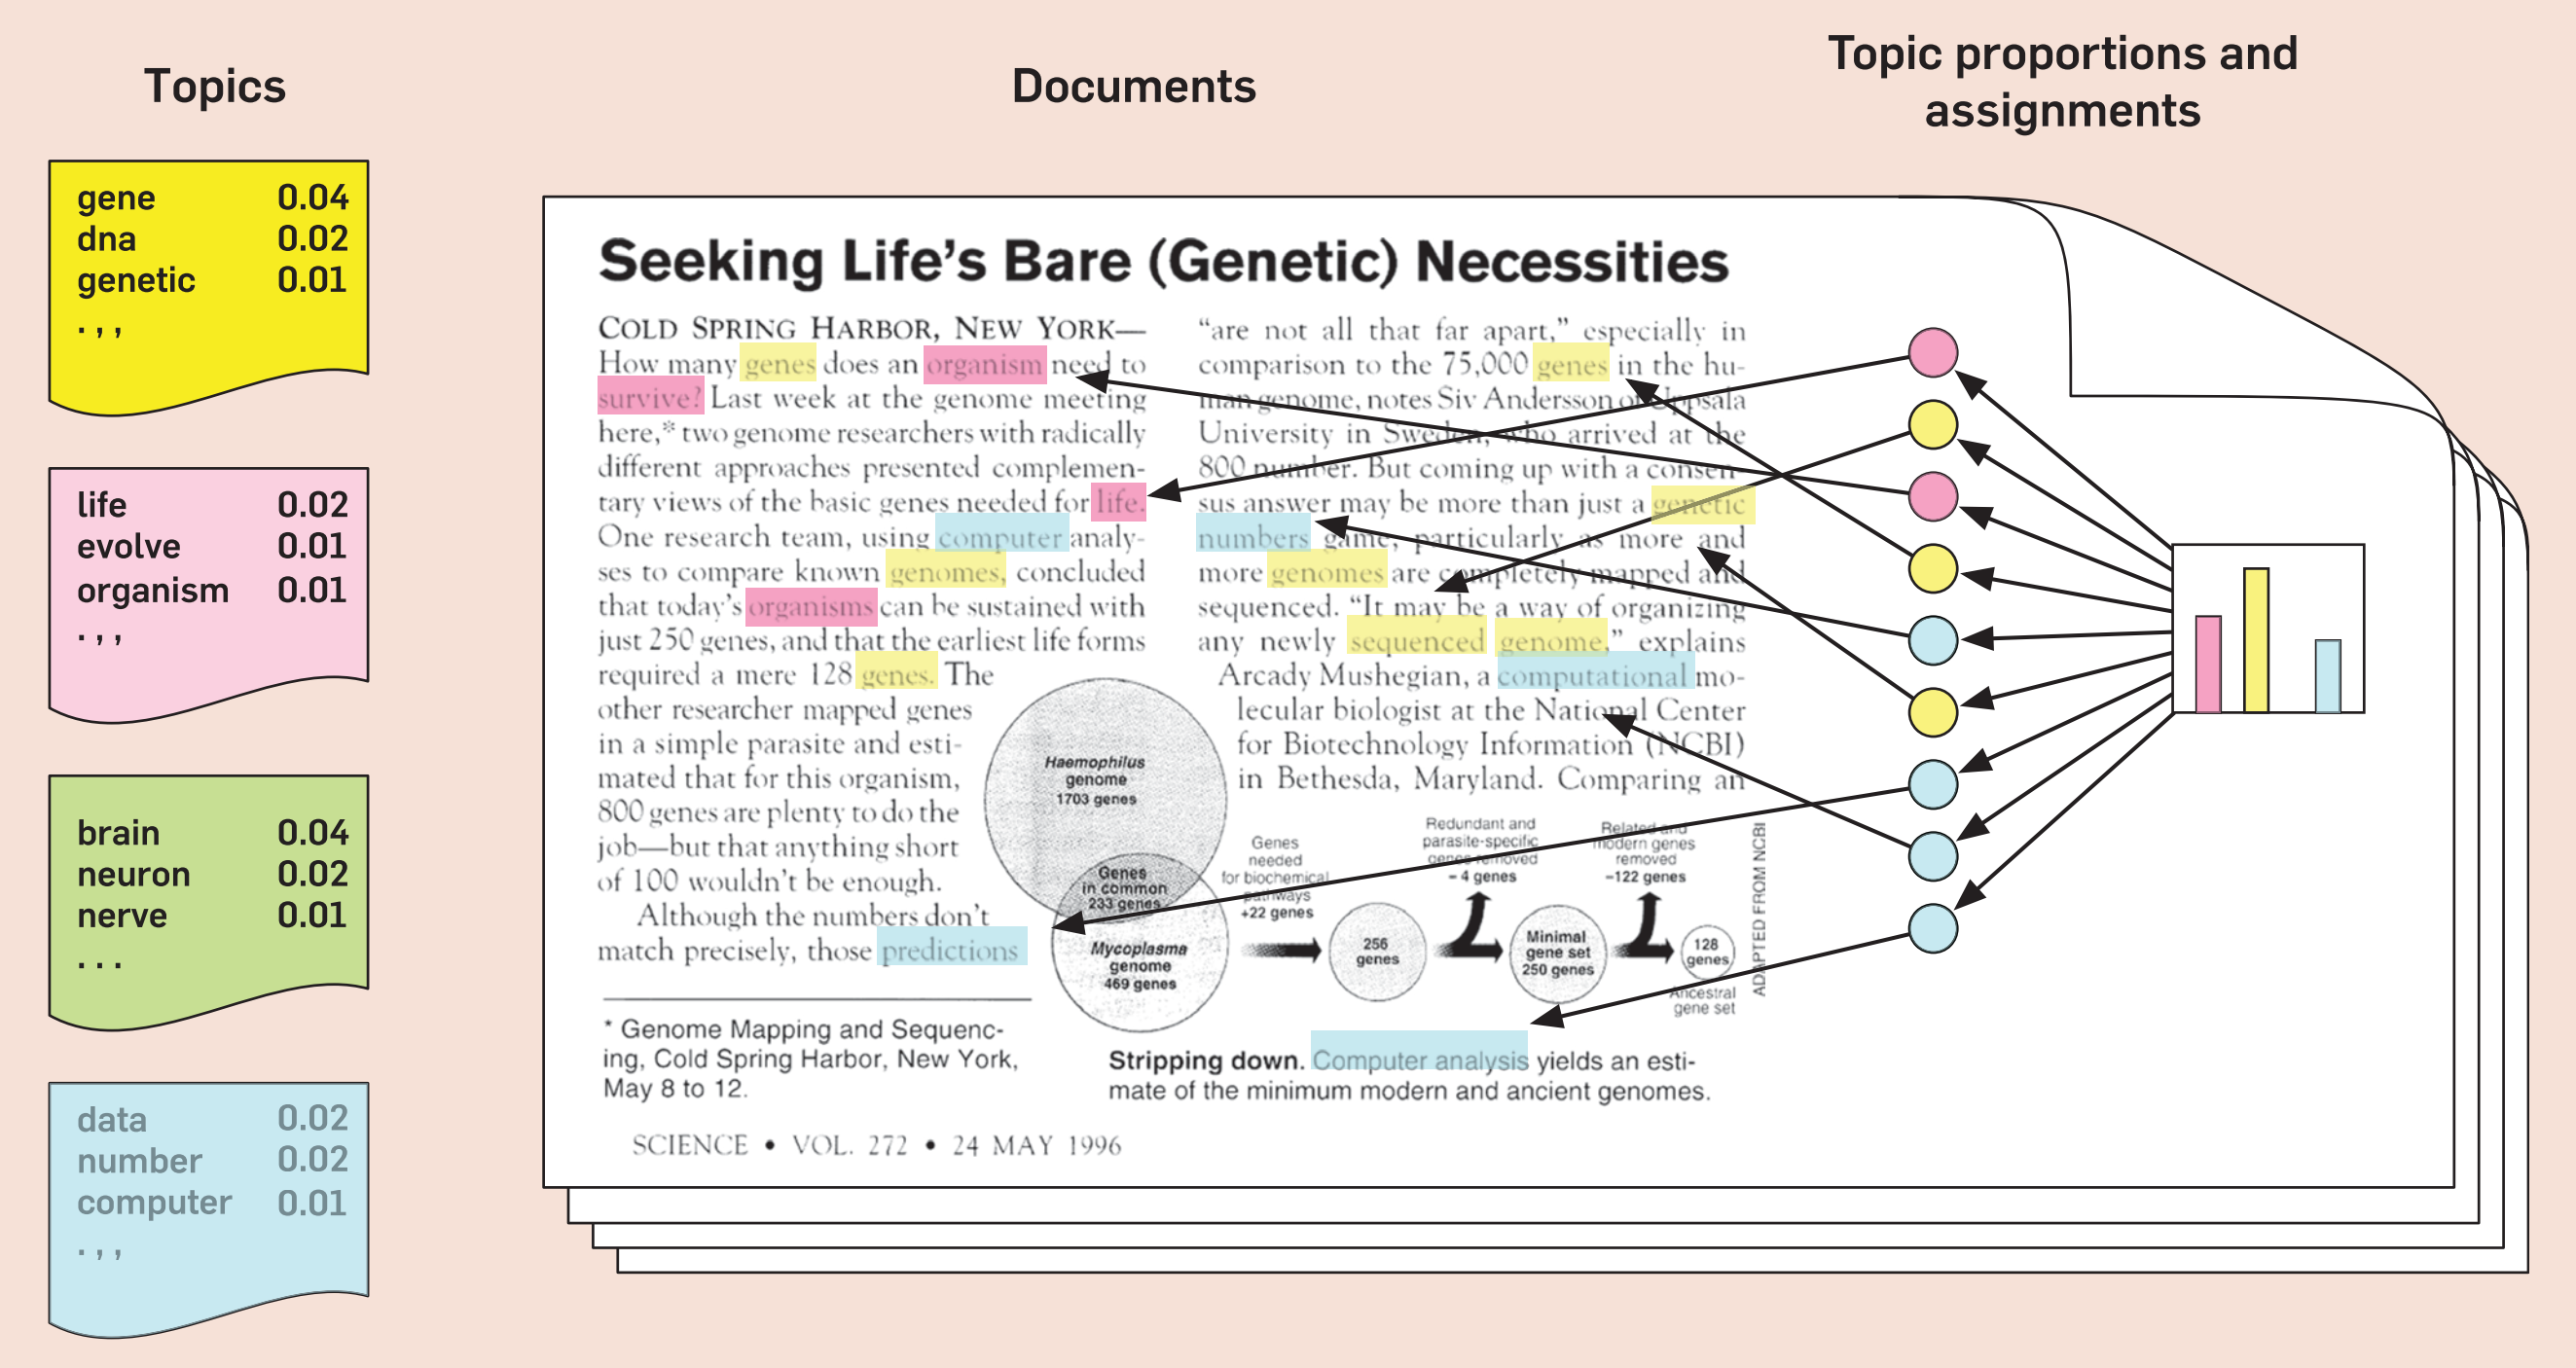
\includegraphics[width=1\textwidth]{figures/topicmodel}
    \caption{The intuition behind Latent Dirichlet Allocation. \cite{kim2019insider}}
\end{figure}
We assume that \textit{every document is a probability distribution over topics} (far right) and \textit{every topic is a probability distribution over words} (far left). The number of topics is a parameter defined by the user at initialization. 
We also assume that each document is generated by the following steps:
\begin{enumerate}
    \item Randomly choose a distribution over topics (the histogram on the right)
    \item Randomly choose the number of words for the document.
    \item For each word:
    \begin{enumerate}
        \item Randomly choose a topic (the colored coins)
        \item Randomly choose a word from the corresponding topic distribution (color from the coin matching the topic color on the left)
    \end{enumerate}
\end{enumerate}
To understand this process mathematically (see fig. \ref{fig:lda}), we reverse engineer a corpus. First, we assume a corpus has $M$ documents and a document has $N$ words $w_n$. The number of words is sampled from a poisson distribution $N\sim Poisson(\xi)$. Every word $w_n$ in a document is sampled from a multinomial distribution $\beta$ conditioned on the topic $z_n$. The topic $z_n$ is again sampled from a multinomial distribution $z_n\sim Multinomial(\theta)$. And at last, the multinomial distribution $Multinomial(\theta)$, that defines the topic distribution for a document, is sampled from a Dirichlet distribution: $\theta\sim Dir(\alpha)$. 
\begin{figure}[H]
    \centering
    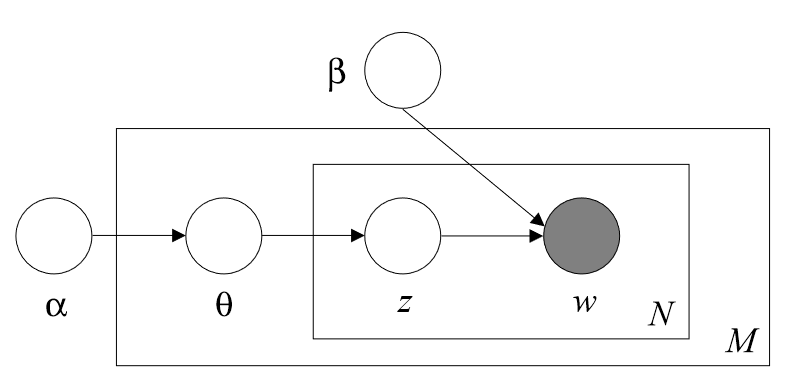
\includegraphics[width=0.8\textwidth]{figures/lda}
    \caption{Graphical model representation of the LDA model. \cite{blei2003latent}}
    \label{fig:lda}
\end{figure}

Simply speaking, if an LDA model is trained on a corpus, what we get are two sets of probability distributions. One set is the topic-word distribution where we get the multinomial distribution of words for every topic. The other is the multinomial distribution of topics for every document. 

With those two sets of distributions, we can make statements about what topics occur within our documents and what words those topics define. We can go even further, with LDA we can generate documents and therefore make assumptions what topics future documents might be about. 

However, a new document may contain words or topics that did not appear in any of the documents in the training corpus. These topics and words would have zero probability in the topic-word distribution. To smooth the multinomial parameters, the document-topic distribution is sampled from a Dirichlet distribution, but not the topic-word distribution. For this reason, we have to modify our LDA model. The modification as seen in fig. \ref{fig:lda_smooth} samples the multinomial topics-word distribution, $\beta$, also from a Dirichlet distribution $\beta\sim Dir(\eta)$.
\begin{figure}[H]
    \centering
    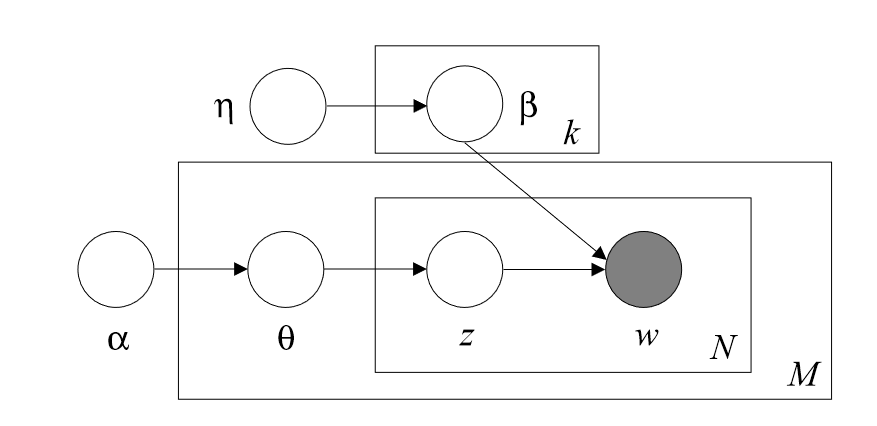
\includegraphics[width=0.8\textwidth]{figures/lda_smooth}
    \caption{Graphical model representation of the smoothed LDA model. \cite{blei2003latent}}
    \label{fig:lda_smooth}
\end{figure}
There are different strategies to train an LDA model. The original paper trains the LDA model through inference with variational Bayes \cite{blei2003latent} but since then there have been various other approaches, e.g. streaming Gibbs sampling \cite{gao2016streaming}, Markov random fields \cite{he2019end}, variational message passing \cite{taylor2021variational}, and many more.

In this work we are using LDA in combination with online variational Bayes \cite{hoffman2010online} which relies on online stochastic optimization. This technique manages to effortlessly analyze a massive amount of documents and can adapt to new documents at a later point in time without being trained from scratch.

% =======================================
\subsection{Neural LDA}
The parameters of the original LDA model have to be learned by variational inference techniques (e.g. EM algorithm for empirical Bayes, Gibbs sampling). This limits the model, especially for new data. Neural LDA proposes a new inference technique (AVITM) \cite{neuralLDA} that utilizes the inference network and does not require running slow variational optimization. To model a Dirichlet distribution with a neural network, they use a Laplace approximation \cite{mackay1998choice} so that the model prior could be assumed Gaussian. With that, the inference network can be defined as a neural network by using the reparametrization trick \cite{kingma2013auto} and the neural network is then able to successfully mimic the probabilistic inference process.  

% =======================================
\subsection{Evaluation and Metrics}
% =======================================
\subsubsection{Metrics of Quality (Topic Coherence)}\label{sec:coherence}
According to João Pedro \cite{topiccoherencemeasures}, topic modeling algorithms are a theoretical technique based on mathematics and statistics. However, a mathematically sound and perfect model does not necessarily reflect an ideal model from a human perspective. For example, a topic modeling algorithm containing the following two topics shows this problem.
\begin{enumerate}
    \item Topic: fish, shark, tuna, sea. \textit{(In our sense a good topic)}
    \item Topic: nurse, brick, cheese, dark. \textit{(In our sense rather a bad topic)}
\end{enumerate}
As a human, one might think the first topic contains more correlating words. On the other hand, for the algorithm, they are probably equal concerning correlating words. Considering our goal to understand data, we want topics that are human-friendly. Misleading and meaningless topics are a consequence of blindly trusting the algorithm. Topic coherence measures aim to put the quality of human perception about the created topics in a number to make the evaluation more feasible. Topic Coherence answers the question of how well a topic fits into a text considering the word combinations (the context) in it. This also means that the measure is not only dependent on the topic itself but also on the original text used for training the topic model. In general, we not only want to judge one topic but all generated topics. Therefore, we have to somehow combine all individual topic scores at the end. 

The topic coherence measure is defined in a pipeline-like structure (segmentation, probability calculation, confirmation measure, aggregation) as shown in fig. \ref{fig:tcm}. Each combination of those components uniquely defines different types of coherence scores. The reference corpus and the topics $t$ are received as inputs and a real valued confirmation measure $c$ is returned. 
\begin{figure}[H]
    \centering
    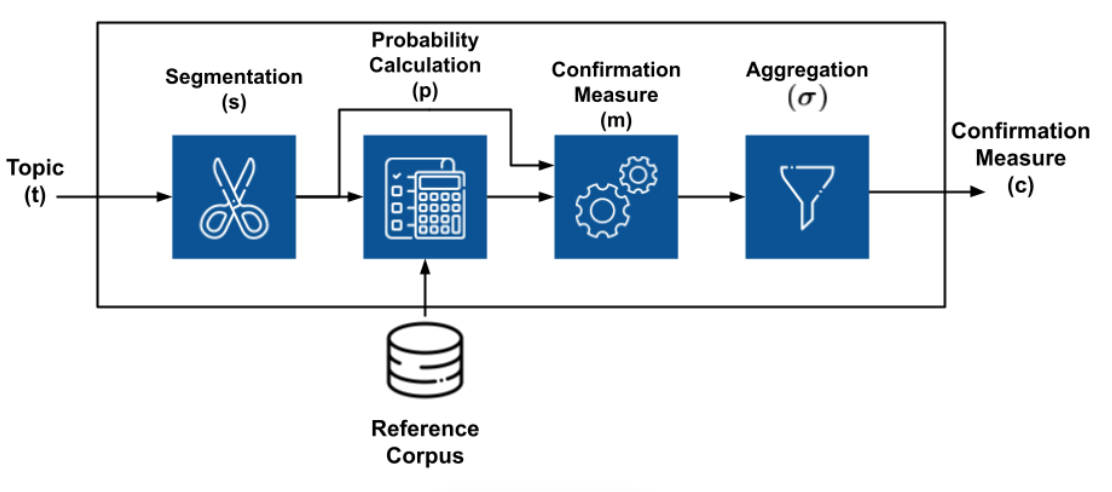
\includegraphics[width=0.9\textwidth]{figures/topiccoherence}
    \caption{General topic coherence measures structure. \cite{topiccoherencemeasures}}
    \label{fig:tcm}
\end{figure}
\textbf{The segmentation part} $s$ creates pairs of word subsets. For example, let $W={w_1,...,w_n}$ be the top-n most probable words of a topic $t$. Then, let $S$ be the set of subset pairs from $W$: $S={(W^{'},W^{*}),W^{'},W^{*}\subseteq W}$. $W^{*}$ is used to confirm $W^{'}$ in the probability calculation part. To get a better grasp of this segmentation let us look at some concrete examples for $W={"seal","egg","fibsh"}$:
\begin{equation}
    \begin{split}
        S^{one}_{one}(W)=\{&(seal,egg),(seal,fibsh),(egg,seal),\\
        & (egg,fibsh),(fibsh,seal),(fibsh,egg)\}
    \end{split}
\end{equation}
\begin{equation}
    \begin{split}
        S^{one}_{all}(W)=\{&(\{seal\},\{egg,fibsh\}),(\{egg\},\{seal,fibsh\}),\\
        & (\{fibsh\},\{seal,egg\})\}
    \end{split}
\end{equation}

\textbf{The probability calculation part} $p$ defines the function used to calculate the probabilities drawn from the corpus. Examples of such functions are the following:
\begin{itemize}
    \item \textbf{P}\textit{bd} (boolean document) calculates the probability as the number of documents the word or words $w$ occur in, divided by the total number of documents.
    \item \textbf{P}\textit{bs} (boolean sentence) calculates the probability as the number of sentences the word or words $w$ occur in, divided by the total number of sentences.
    \item \textbf{P}\textit{bsw} (boolean sliding window) calculates the probability as the number of sliding windows the word or words $w$ occur in, divided by the total number of sliding windows.
\end{itemize}
\textbf{The confirmation measure part} $m$ calculates a score by evaluating the probability function over the segmentations $S$ from the previous part. A low confirmation measure implicates that the words in $W^{'}$ are disconnected with the words in $W^{*}$ and vice versa (see fig. \ref{fig:tcp}). 
\begin{figure}[H]
    \centering
    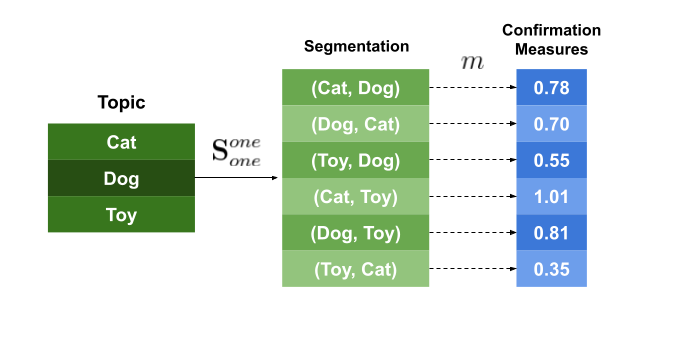
\includegraphics[width=0.9\textwidth]{figures/coherenceproba}
    \caption{Example of application of a confirmation measure $m$. \cite{topiccoherencemeasures}}
    \label{fig:tcp}
\end{figure}
There are two different types of confirmation measures:

\textit{Direct confirmation measures} use the subsets $W^{'}$ and $W^{*}$ to calculate the resulting score. E.g.:
\begin{equation}
    m_r(S_i)=\frac{P(W^{'},W^{*})}{P(W^{'})P(W^{*})}
\end{equation}
\begin{equation}
    m_{lr}(S_i)=log\frac{P(W^{'},W^{*})+\epsilon}{P(W^{'})P(W^{*})}
\end{equation}
\begin{equation}
    m_c(S_i)=\frac{P(W^{'},W^{*})}{P(W^{*})}
\end{equation}

\textit{Indirect confirmation measures} use the subset $W^{'}$ and $W^{*}$ separately to build a vector for all the words $W$ (see eq. \ref{eq:confmeas1}, \ref{eq:confmeas2}).
\begin{equation}
    \vec{v}_m(W^{'})=\left\{\sum_{w_i\in W^{'}}{m(w_i,w_j)}\right\}_{j=1,2,...,|W|}
    \label{eq:confmeas1}
\end{equation}
\begin{equation}
    \vec{v}_m(W^{'})=\left\{\sum_{w_i\in W^{'}}{m(w_i,w_j)}\right\}_{j=1,2,...,|W|}
    \label{eq:confmeas2}
\end{equation}
Those two vectors are combined with, for example, the cosine similarity function (see eq. \ref{eq:cos}).
\begin{equation}
    \tilde{m}_{cos}(W^{'},W^{*})=s_{cos}(\vec{v}_m(W^{'}),\vec{v}_m(W^{*}))
    \label{eq:cos}
\end{equation}
The idea behind the indirect confirmation measure is to find relations that the direct method could not.

\textbf{The aggregation part} $\sigma$ combines all previously calculated values into one. This value is the final topic coherence score and can be, for example, the arithmetic mean.

Currently, the score that has the highest correlation with all available human topic-ranking data is the coherence score $C_v$ \cite{syed2017full}. The type of the coherence score, as mentioned before, is uniquely defined by the segmentation, the probability calculation, the confirmation measure and the aggregation:
\begin{itemize}
    \item $S_{set} = \{(W', W^{*})\mid W' = \{w_i\}; w_{i} \in W; W^{*} = W\}$
    \item \textbf{P}\textit{bsw} - Boolean Sliding Window
    \item $\phi_{S_i}(\vec{u},\vec{w})=\frac{\sum_{i=1}^{|W|}{\vec{u}_i}\cdot\vec{w}_i}{\|\vec{u}\|_2\cdot\|\vec{w}\|_2},\;$ with $\;
           \vec{v}(W^{'})=\left\{\sum_{w_i\in W^{'}}{\textbf{NPMI}(w_i,w_j)^{\gamma}}\right\}_{j=1,...,|W|}\;$ and 
            $\;\textbf{NPMI}(w_i,w_j)^{\gamma}=\left(\frac{\text{log}\frac{P(w_i,w_j)+\epsilon}{P(w_i)\cdot P(w_j)}}{-\text{log}(P(w_i,w_j)+\epsilon}\right)$
    \item $\sigma=$ The arithmetic mean
\end{itemize}

A full insight in topic coherence measures with more examples of each part can be found in \textit{Exploring the Space of Topic Coherence Measures} by Röder et al. \cite{roder2015exploring}

% =======================================
\subsubsection{Metrics of Differences Between Models (Distance)}\label{sec:diffmet}
Topic models generate probability distributions and one way to compare those models with each other is to measure the similarity between them. We can do this by using the Jensen-Shannon distance. The Jensen-Shannon distance is the square root of the Jensen-Shannon divergence, also known as the information radius or total divergence to the average. The Jensen-Shannon divergence \cite{fuglede2004jensen} is based on the Kullback-Leibler divergence ($D_{KL}$) with the difference that it is symmetric and it always has a finite value. 
\begin{equation}
    JSD(P||Q)=\frac{1}{2}D_{KL}\left(P\left|\left|\frac{1}{2}(P+Q)\right.\right.\right)+\frac{1}{2}D_{KL}\left(Q\left|\left|\frac{1}{2}(P+Q)\right.\right.\right),
\end{equation}
with $D_{KL}(P||Q)$ denoting the relative entropy of $P$ with respect to $Q$.

The more similar the two distributions $P$ and $Q$ are, the closer to zero the resulting value is. The evaluation between two topic models requires both to have been trained with the same vocabulary. The vocabularies have to be exactly the same, including the positions of the words. Otherwise, additional and very tedious coding is required.

Furthermore, the topics of two topic models are not guaranteed to match the same topic IDs (1-1, 2-2, etc.). Therefore, the result is going to be a matrix ($M_{i,j}$ with $i,j\in[0,...,t]$, where $t=\textit{num topics}-1$), where all topics are compared to each other. The matching topics are then found by the lowest score for every line (or row). 